\part{Armado}
Debido a la gran parte de elementos que constituyen el entrenador y de la multiplicidad de tareas a realizar, así como los saberes a trabajar con los alumnos; el armado de la totalidad del entrenador se lleva a cabo entre desde el 3ero año hasta el 5to año de la carrera.   
\section{Gabinete}
\begin{multicols}{2}
Realizado en madera de pino y placas de MDF previamente cortada a medida, se le entrega a los alumnos que se encuentran cursando el 3er año de la carrera manera que los mismos arman el gabinete y le dan un acabado protector en barniz o de otro tipo a gusto.
\begin{figure}[H]
	
\includegraphics[trim=18cm 2cm 18cm 2cm,clip=true,width=0.5\textwidth]{GabineteRender}\caption{Gabinete de madera del entrenador digital.}\label{GabineteRender}

\end{figure}

\end{multicols}
\subsection{Croquis}
El croquis solo debe de tomarse como una guía, ya que los materiales entregados por el proveedor suelen variar en el espesor y el ancho, por otro lado el largo de las varillas se obtiene en la escuela. 

\begin{figure}[h!]
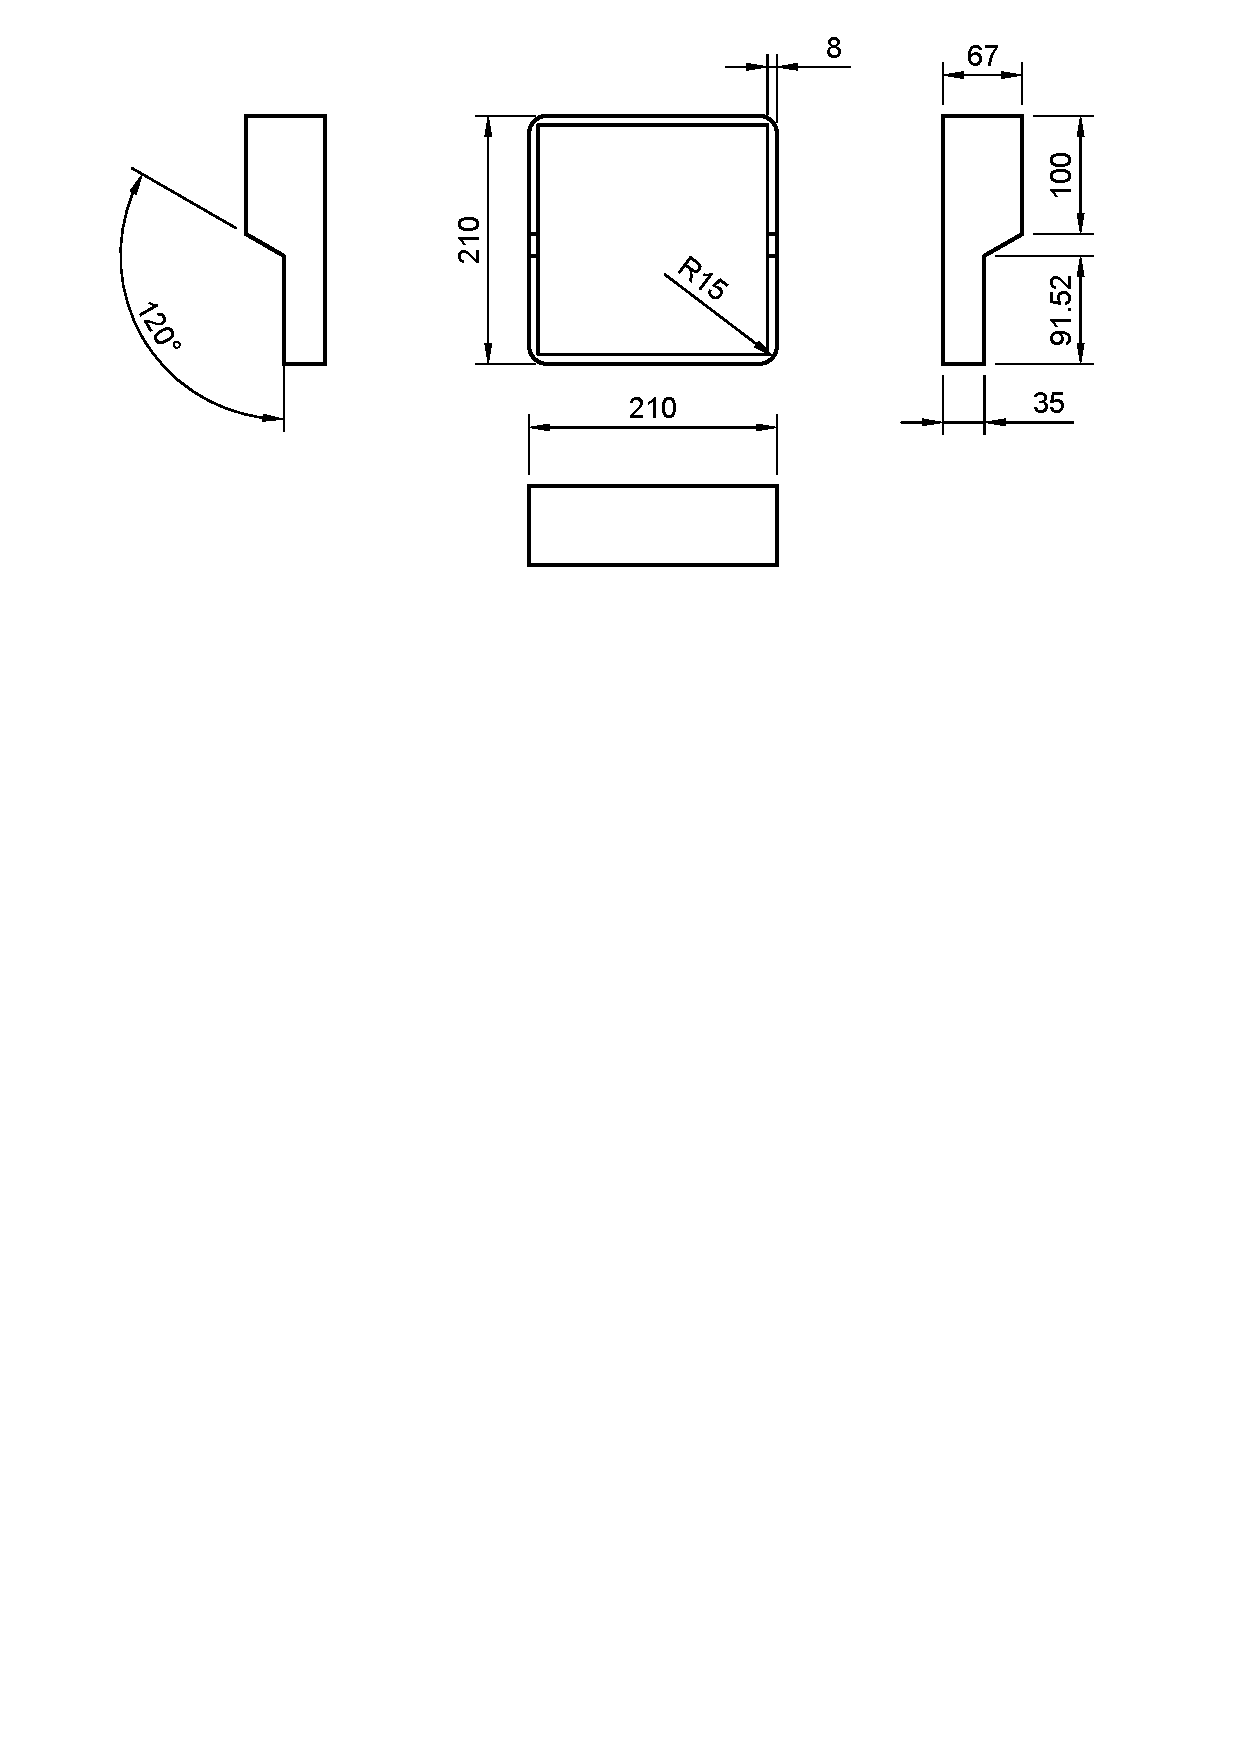
\includegraphics[trim=1cm 20cm 1cm 0cm, clip=true,  width=\textwidth]{GabineteMaderav1}\caption{Croquis del gabinete de madera.}\label{CroquisdelGabinetedeMadera}
\end{figure}
\subsection{Lista de materiales}
Para completar el gabinete se requiere de los siguientes recorte de madera:
\begin{itemize}
	\item Tres laterales de 210mm x 33mm x 8mm (tolerancia 2mm).
	\item Dos laterales de 118mm x 33mm x 8mm (tolerancia 2mm).
	\item Una tapa trasera de 210mm x 67mm x 8mm (tolerancia 2mm).
	\item Una tapa inferior o base de 210mm x 210mm x 3mm.
	\item Una tapa superior o frente de 210mm x 100mm x 3mm.
	 
\end{itemize}

Mayor información se puede encontrar en el blog de la institución dentro de la lista de trabajos correspondientes al 3er año para el módulo de Sistemas Tecnológicos. 


\section{Fuente de alimentación}
Se realiza en el tercer año de la carrera, los alumnos en esta etapa aún no conocen los componentes de uso frecuente en electrónica ni las técnicas de soldado y de producción de placas, por esto se trabaja con la fuente durante los dos primeros trimestres del año en los cuales se van desarrollando las primeras capacidades (ver expectativas de logro \ref{Exp1} y \ref{Exp2}).

la placa de la fuente se realiza siguiente el circuito de la figura \ref{CircuitoFuente}.

\begin{figure}[H]
	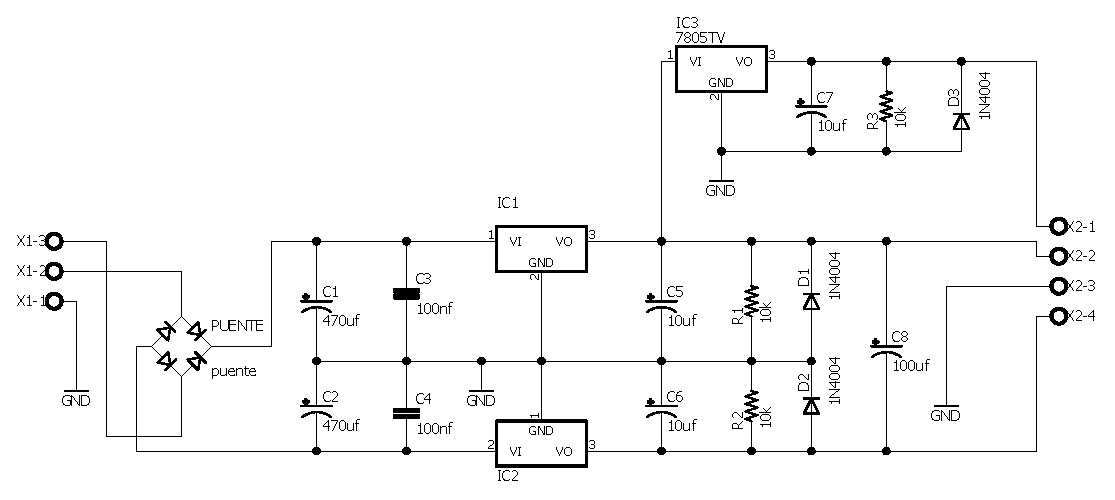
\includegraphics[width=\textwidth]{CircuitoFuente.eps}\caption{Circuito esquemático de la fuente}\label{CircuitoFuente}
\end{figure}
\begin{figure}[H]
	\begin{tikzpicture}
	
	\node[]{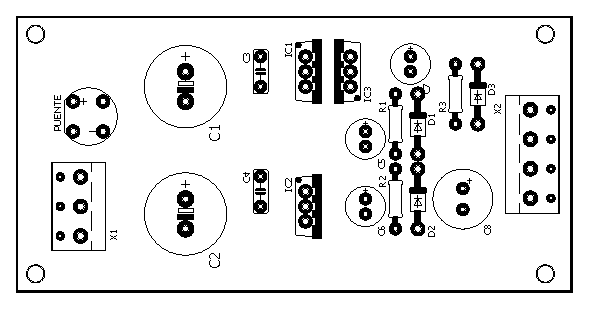
\includegraphics[width=\textwidth]{VistaComponentes.eps}};
	\draw (-7,-1.5) node[rotate=90](Entrada){\Large Entrada};
	\draw (8,0) node[rotate =90](Salida){\Large Salida};
	\end{tikzpicture}\caption{Vista de componentes sobre la placa de la fuente}\label{LadoComponentesFuente}
\end{figure}

Se puede observar que la fuente consta de tres valores de tensión de salida para que los alumnos tengan al finalizar el trabajo una herramienta versatil. Existe un documento para ampliar la información necesaria para llevar a cabo la construcción de la fuente en el blog de la escuela.

\section{Placa Principal}
La placa principal es el entrenador propiamente dicho y consta a su vez de dos partes; la paca base y la placa superior. Ambas placas son producidas por los alumnos de; 7mo año de la carrera en el marco del plan de prácticas internas dentro del laboratorio de diseño electrónico.

	



